\documentclass[10pt]{article}
\usepackage[utf8]{inputenc}
\usepackage{amscd}
\usepackage{amsmath}
\usepackage{amssymb}
\usepackage{amsthm}
\usepackage{listings}
\usepackage{enumerate}
\usepackage{graphicx}

\graphicspath{{images/}}

\textwidth=15cm \textheight=22cm \topmargin=0.5cm \oddsidemargin=0.5cm \evensidemargin=0.5cm

\newcommand{\sk}{\vskip 10mm}
\newcommand{\bb}[1]{\mathbb{#1}}
\newcommand{\ra}{\rightarrow}

\theoremstyle{plain}
\newtheorem{problem}{Problem}
\newtheorem{lemma}{Lemma}[problem]

\theoremstyle{remark}
\newtheorem{tpart}{}[problem]
\newtheorem*{ppart}{}

\begin{document}

\begin{problem} %1
  
\end{problem}

\[S_3 \cong \langle a,b,c | a^2,b^2,c^2,(ab)^3,(ac)^3 \rangle\]

We can identify $a$ with $(1\ 2)$, $b$ with $(2\ 3)$, and
$c$ with $(1\ 3)$.

\sk

\begin{problem} %2
  
\end{problem}

\begin{proof}
  Start with $\langle a,b| a^4=1,b^2=1,bab^{-1}=a^{-1}\rangle$. Then the elements of this group
  are
  \[ e,a,a^2,a^3,b,ba^2,ba^3,ab,a^2b,a^3b,bab,aba,\ldots \]
  However using the relations above $bab=bab^{-1}=a^{-1}$ and similarly
  we also have $aba=b$. In addition we have $b=b^{-1}$ and as such $ba=a^{-1}b$
  which implies that $ba^i=a^{-i}b$ collapsing more elements until we are left with
  \[ e,a,a^2,a^3,b,ba,ba^2,ba^3 \]
  showing that the group is of order 8.

  Now consider the symmetries of a square with vertices labeled clockwise $1,2,3,4$.
  Then the symmetries consist of 8 permutations
  \[ e,(1\ 2\ 3\ 4),(1\ 4)(2\ 3),(4\ 3\ 2\ 1),(1\ 2)(3\ 4),(2\ 4),(1\ 4)(2\ 3),(1\ 3)\]
  Define $\rho:=(1\ 2\ 3\ 4)$ and $r:=(1\ 2)(3\ 4)$. It can be seen that $\rho$ and $r$
  generate the others. Note that since $\rho$ is a 4-cycle and
  $r$ is a product of disjoint transpositions that $\rho^4=e$ and $r^2=1$.
  In addition if we consider $r\rho r^{-1}$ we have
  \[ r\rho r^{-1}=(1\ 2)(3\ 4)(1\ 2\ 3\ 4)(1\ 2)(3\ 4)=(4\ 3\ 2\ 1)=\rho^{-1}\]
  Since there are eight permutations of the square and their generators fulfill the
  same relations we can conclude that
  $( a,b| a^4=1,b^2=1,bab^{-1}=a^{-1})$ is isomorphic to the group of symmetries of the
  square.
\end{proof}

\sk

\begin{problem} %3
  
\end{problem}

\begin{proof}
  Define a map $\varphi:G\rightarrow H$ by
  \[ \varphi(a)=xyx,\quad \varphi(b)=xy\]
  and define $\varphi$ for the rest of the elements of $G$ by concatenation.

  We will show it is a homomorphism by showing that it preserves the relation
  $a^2=b^3$.
  \begin{align*}
    \varphi(a)^2&= xyxxyx\\
         &= xyxyxy\\
         &= (xy)^3\\
         &= \varphi(b)^3
  \end{align*}
  proving that $\varphi$ is a homomorphism.

  Now we will show that $\varphi(a)$ and $\varphi(b)$ are also generators of $H$. This
  will allow us to define $\varphi^{-1}$ by simply reversing the map which will
  show that $\varphi$ is an isomorphism.

  For $x$ we have
  \[ y = y^{-1}x^{-1}xyx = (xy)^{-1}xyx = \varphi(b)^{-1}\varphi(a)\]
  Then for $y$ it is
  \[ y = yxyy^{-1}x^{-1}=xyx(xy)^{-1} =\varphi(a)\varphi(b)^{-1}\]
  Since we can reach the generators of $H$ from $\varphi(a)$
  and $\varphi(b)$ they are also generators of $H$. 
  Therefore there is a well-defined
  inverse $\varphi^{-1}$ by reversing the map which shows
  that $\varphi$ is an isomorphism.

  Therefore the groups $G$ and $H$ are isomorphic.
\end{proof}

\sk

\begin{problem} %4
  
\end{problem}

\begin{proof}
  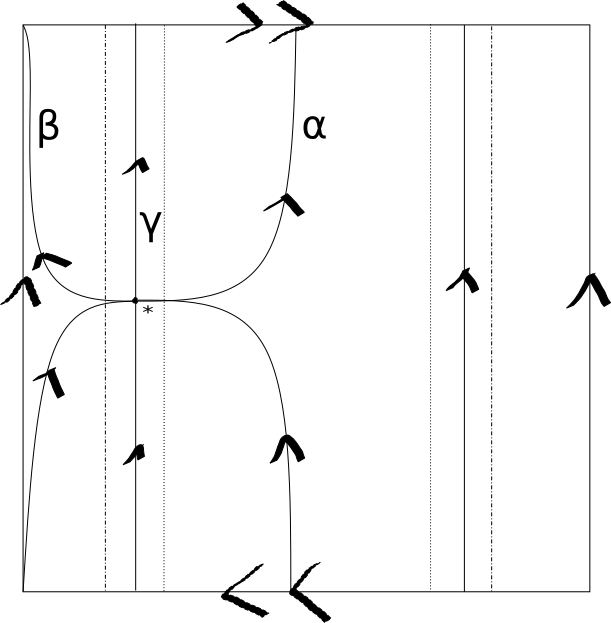
\includegraphics[scale=.5]{klein}

  We will show that the fundamental of the Klein bottle $\pi_1(K,*)$ is
  isomorphic to \\$\langle a,b|aba^{-1}b=1\rangle$. First as above we decompose
  $K$ into $U$ and $V$ where $U$ lies in the center between the dashed dotted lines
  and $V$ lies on the outer edges between the dotted lines. Then
  $U,V$ and $U\cap V$ can be seen to be M\"obius strips.
  The M\"obius strips are each homotopy equivalent to a circle. Therefore
  the fundamental groups of $U,V,$ and $U\cap V$ are
  \[ \pi_1(U,*)\cong \pi_1(V,*)\cong \pi_1(U\cap V,*)\cong \pi_1(S^1,*)\cong\bb{Z}\]

  Next we examine the generators for each of the fundamental groups. The generators
  for $\pi_1(U,*),\pi_1(V,*),$ and $\pi_1(U\cap V,*)$ are $[\alpha],[\beta],$ and $[\gamma]$ respectively.
  Take the inclusion maps $i:U\cap V\rightarrow U$ and $j:U\cap V \rightarrow V$. Then
  $i_*([\gamma])=[\alpha]^2$ and similarly $j_*([\gamma])=[\beta]^2$. We can see this because if we were
  to project $\gamma$ and $\alpha$ (or $\beta$) onto a circle we would have $\gamma$ go around twice as
  many times as $\alpha$. Then by the Seifert-van Kampen Theorem we have
  \[\pi_1(K,*)=\langle [\alpha],[\beta] | i_*([\gamma])j_8([\gamma])^{-1}=1 \rangle\cong\langle [\alpha],[\beta]|[\alpha]^2[\beta]^{-2}=1\rangle \cong \langle x,y| x^2=y^2\rangle\]

  Now we will show that $\langle x,y| x^2=y^2\rangle\cong \langle a,b|aba^{-1}b=1\rangle$. First note that we
  can rewrite $aba^{-1}b=1$ as $bab=a$ via
  \[ aba^{-1}=b^{-1}\Rightarrow ab=b^{-1}a\Rightarrow bab=a \]
  Define a map $\varphi$ such that
  \[ \varphi(x)=ba,\quad \varphi(y)=a\]
  where we define $\varphi$ on other elements by concatenation.
  Then we can show that $\varphi$ is a homomorphism by showing it preserves the relation
  $x^2=y^2$ via
  \begin{align*}
    \varphi(x)^2 &= baba\\
          &= a^2\\
          &= \varphi(y)^2
  \end{align*}

  Next we will show that we can reach both generators $a,b$ which from the same reasoning
  as problem $3$ will show that $\varphi$ is an isomorphism. We can express $a$ immediately
  as $\varphi(y)=a$. For $b$ we have $\varphi(x)\varphi(y)^{-1}=baa^{-1}=a$. It then follows that $\varphi$
  is an isomorphism.

  Therefore the fundamental group of the Klein bottle has presentation
  $\langle a,b|aba^{-1}b=1\rangle$.
\end{proof}

\sk

\begin{problem} %5
  
\end{problem}

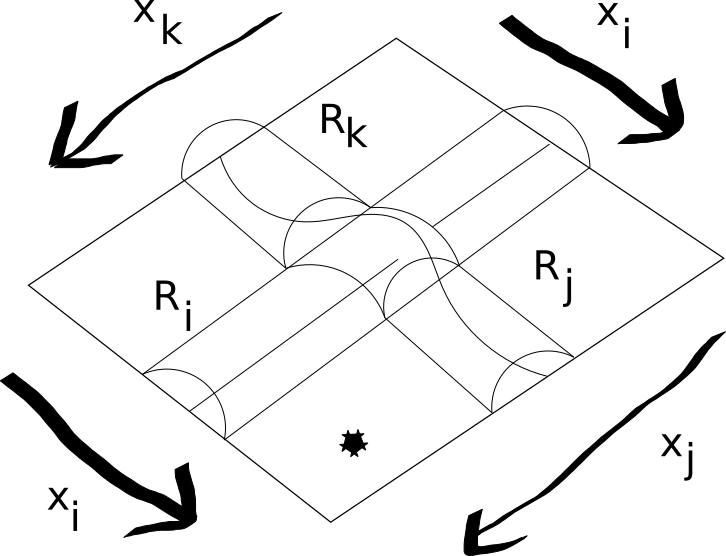
\includegraphics[scale=.5]{wirt}

\begin{proof}
  \begin{itemize}
  \item[a)]
    First we look at the space $T$ with the $R$s attached. Going along
    $T$ and passing through $R_n$ to return to the basepoint is a generator
    which we will call $x_n$. For each arc $\alpha_i$ there will be a
    corresponding generator $x_i$. Given a crossing we can frame it as in
    the drawing above. Then if we go along the loop $x_i$ with the orientation
    listed followed by $x_j,x_i^{-1},$ and then $x_k^{-1}$ we can pull
    the loop back to the constant loop obtaining the relation $x_ix_jx_i^{-1}x_k^{-1}=1$.
    This can be rewritten as $x_ix_jx_i^{-1}=x_k$. Then the presentation
    of $\pi_1(\bb{R}^3\setminus K)\cong\langle x_1,\ldots,x_m|x_ix_jx_i^{-1}=x_k \text{\ for each crossing}\rangle$
    where $m$ is the number of crossings.
  \item[b)] Since the presentation will consist solely of relations of the
    form $x_ix_jx_i^{-1}=x_k$ the Abelianization of the group would reduce
    all such relations to the form $x_ix_i^{-1}x_j=x_jx_k$. However since $K$ is a knot each
    distinct arc will be related to each other either directly or through
    transitivity. This means that all generators will be equivalent leaving
    us with $\bb{Z}$ as the Abelianization of $\pi_1(\bb{R}^3\setminus K)$.
  \end{itemize}
\end{proof}

\sk

\begin{problem} %6
  
\end{problem}

\begin{proof}
  
\includegraphics[scale=.2]{trefoil}

  Using Problem $5$ we can deduce that the presentation of the group is
  \[\langle a,b,c | aba^{-1}=c,bcb^{-1}=a,cac^{-1}=b\rangle\]
  However we can simplify this
  presentation by plugging the first relation into the latter two to get
  \begin{align*}
    bcb^{-1} &= a\\
    baba^{-1}b^{-1} &= a \\
    bab &= aba
  \end{align*}
  and similarly
  \begin{align*}
    cac^{-1} &= b\\
    aba^{-1}aab^{-1}a^{-1} &= b \\
    abab^{-1}a^{-1} &= b\\
    aba = bab
  \end{align*}
  Since we get the same relation and have removed all instances of the generator
  $c$ we can safely trim down our original presentation to
  $\langle a,b| aba=bab\rangle$.

  Therefore the fundamental group of the trefoil knot is isomorphic to
  $\langle x,y| xyx=yxy\rangle$. Moreover this group is not Abelian as
  $xy = yxyx^{-1}$. It then follows that the trefoil knot is not equivalent to the
  unknot as the fundamental group of the unknot is Abelian.
\end{proof}

\sk

%%%%%%%%%%%%%%%%%%%%%%%%%%%%%%%%%%%%%%%%%%%%%%%%%%%%%%%%%%%%%%%%%%%%%%%%%%%%%
\end{document}
